% Chapter 6 — Web application (system artifact).
\section{Web Application}

The system is deployed as a two-tier web application (Figure~\ref{fig:arch}).

\begin{figure}[t]
\centering
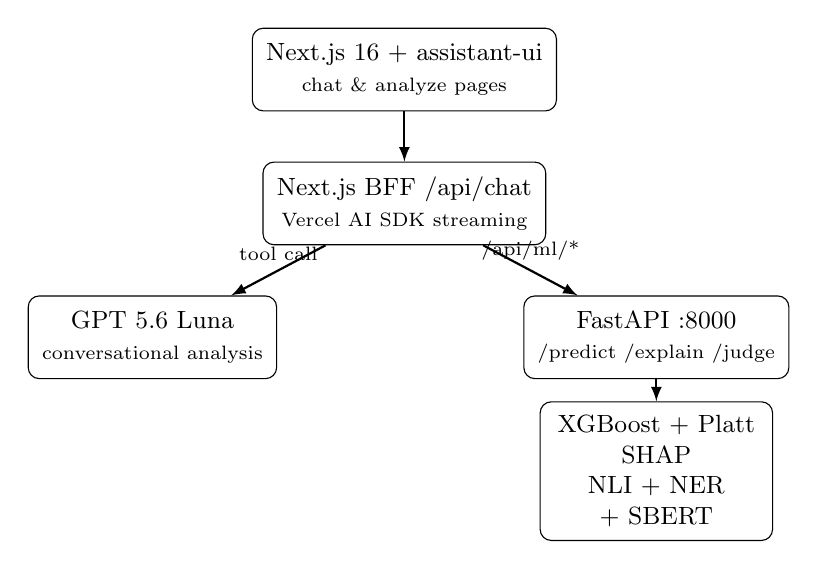
\begin{tikzpicture}[
    box/.style={draw, rounded corners=4pt, minimum height=1.05cm, inner sep=5pt, align=center, font=\small},
    arrow/.style={-latex, thick},
]
\node[box] (ui) at (0, 0) {Next.js 16 + assistant-ui\\\scriptsize chat \& analyze pages};
\node[box] (bff) at (0, -1.7) {Next.js BFF /api/chat\\\scriptsize Vercel AI SDK streaming};
\node[box] (llm) at (-3.2, -3.4) {GPT 5.6 Luna\\\scriptsize conversational analysis};
\node[box] (api) at (3.2, -3.4) {FastAPI :8000\\\scriptsize /predict /explain /judge};
\node[box, text width=2.6cm] (ml) at (3.2, -5.1) {XGBoost + Platt\\SHAP\\NLI + NER + SBERT};
\draw[arrow] (ui) -- (bff);
\draw[arrow] (bff) -- node[above, font=\scriptsize]{tool call} (llm);
\draw[arrow] (bff) -- node[above, font=\scriptsize]{/api/ml/*} (api);
\draw[arrow] (api) -- (ml);
\end{tikzpicture}
\caption{HaluRISC system architecture: the Next.js backend-for-frontend proxies ML requests to FastAPI and streams LLM chat with tool-generated UI widgets.}
\label{fig:arch}
\end{figure}

The FastAPI backend loads all artifacts (model, calibrator, SHAP explainer, NLI/NER/embedding models) once at startup and exposes \texttt{/predict}, \texttt{/explain}, \texttt{/judge}, and \texttt{/health} with Pydantic validation. The Next.js frontend provides (i) a chat mode using assistant-ui Thread primitives where GPT 5.6 Luna calls the analysis tool and the risk gauge and SHAP chart render directly inside the streaming message; (ii) an analyze mode with an animated semicircular risk gauge, calibrated score, and SHAP contribution bars; (iii) an experiment dashboard rendering live results from \texttt{artifacts/results/}; and (iv) an about page.

Figure~\ref{fig:screens} shows the three analysis cases: a clearly hallucinated answer (high risk), a grounded answer (low risk), and a borderline answer near 50\%.

\begin{figure}[t]
\centering

\includegraphics[width=0.62\textwidth]{hallucinated_date.png}\\
\vspace{0.3em}

\includegraphics[width=0.62\textwidth]{grounded_correct.png}
\caption{Analyze page: hallucinated-date case (high risk) and grounded case (low risk) with SHAP contribution charts.}
\label{fig:screens}
\end{figure}
